\documentclass[12pt,letterpaper]{report}

% ============================================
% PAQUETES NECESARIOS
% ============================================
\usepackage[utf8]{inputenc}
\usepackage[spanish,es-tabla]{babel}
\usepackage{mathptmx}  % Times New Roman
\usepackage[left=3cm, right=3cm, top=3cm, bottom=3cm]{geometry}
\usepackage{setspace}
\usepackage{titlesec}
\usepackage{graphicx}
\graphicspath{{img/}}  % Carpeta de imágenes
\usepackage{float}  % Para posicionar figuras con [H]
\usepackage{hyperref}
\usepackage{fancyhdr}
\usepackage{array}
\usepackage{longtable}
\usepackage{amsmath}
\usepackage{amssymb}
\usepackage[numbers]{natbib}
\usepackage{caption}
\usepackage{tocloft} % Paquete para personalizar índices


% ============================================
% CONFIGURACIÓN DE FORMATO
% ============================================

% Interlineado sencillo
\singlespacing

% Configuración de párrafos: justificado con espaciado 12pt antes y después
\setlength{\parindent}{0pt}
\setlength{\parskip}{5pt}

% Configuración de títulos según especificaciones
% Título 1 (Capítulo): Times New Roman Negrita 14
\titleformat{\chapter}[display]
  {\normalfont\bfseries\fontsize{14}{16}\selectfont}
  {\thechapter.}{10pt}{}
\titlespacing*{\chapter}{0pt}{0pt}{12pt}

% Título 2 (Sección): Times New Roman Negrita 13
\titleformat{\section}
  {\normalfont\bfseries\fontsize{13}{15}\selectfont}
  {\thesection}{1em}{}
\titlespacing*{\section}{0pt}{12pt}{12pt}

% Título 3 (Subsección): Times New Roman Negrita 12
\titleformat{\subsection}
  {\normalfont\bfseries\fontsize{12}{14}\selectfont}
  {\thesubsection}{1em}{}
\titlespacing*{\subsection}{0pt}{12pt}{12pt}

% Configuración de numeración de páginas
\pagestyle{fancy}
\fancyhf{}
\fancyfoot[C]{\thepage}
\renewcommand{\headrulewidth}{0pt}

% Configuración de figuras y tablas
\captionsetup[figure]{font=small,labelfont=bf}
\captionsetup[table]{font=small,labelfont=bf,position=below}

% ============================================
% INICIO DEL DOCUMENTO
% ============================================
\begin{document}

% Numeración romana para preliminares
\pagenumbering{roman}
\setcounter{page}{1}

% ============================================
% PORTADA
% ============================================
\begin{titlepage}
\centering

{\fontsize{14}{16}\selectfont\bfseries DISEÑO E IMPLEMENTACIÓN DE UNA PLATAFORMA DE ESTABILIZACIÓN PARA UNA BICICLETA UTILIZANDO UN VOLANTE DE INERCIA\par}
{\fontsize{12}{14}\selectfont Nombre\_Empresa\par}
\begin{center}

\includegraphics[width=0.35\textwidth]{image1.jpeg}
\vfill
\end{center}{\fontsize{12}{14}\selectfont\bfseries Autores\par}
{\fontsize{12}{14}\selectfont Jeferson Hernan Hernandez Moreno\par}
{\fontsize{12}{14}\selectfont Fabian Andrés Reyes Romero\par}

\vfill

{\fontsize{12}{14}\selectfont\bfseries UNIVERSIDAD DISTRITAL FRANCISCO JOSÉ DE CALDAS\par}
{\fontsize{12}{14}\selectfont Facultad Tecnológica\par}
{\fontsize{12}{14}\selectfont Ingeniería en Control\par}



{\fontsize{12}{14}\selectfont Bogotá D.C. Enero, 2026\par}

\end{titlepage}

% ============================================
% CONTRAPORTADA
% ============================================
\newpage
\begin{titlepage}
\centering

{\fontsize{14}{16}\selectfont\bfseries DISEÑO E IMPLEMENTACIÓN DE UNA PLATAFORMA DE ESTABILIZACIÓN PARA UNA BICICLETA UTILIZANDO UN VOLANTE DE INERCIA\par}
{\fontsize{12}{14}\selectfont Nombre\_Empresa\par}
\centering

\includegraphics[width=0.35\textwidth]{image1.jpeg}
\vfill



{\fontsize{12}{14}\selectfont\bfseries Autores\par}
{\fontsize{12}{14}\selectfont Jeferson Hernan Hernandez Moreno Código: 20201383013\par}
{\fontsize{12}{14}\selectfont jhhernandezm@udistrital.edu.co\par}
{\fontsize{12}{14}\selectfont Fabian Andrés Reyes Romero Código: 20201383011\par}
{\fontsize{12}{14}\selectfont fareyesr@udistrital.edu.co\par}
\vfill


{\fontsize{12}{14}\selectfont\bfseries INFORME FINAL DE PASANTÍA\par}


{\fontsize{12}{14}\selectfont Presentado para optar al título de: Ingeniero en Control y Automatización\par}

\vfill

{\fontsize{12}{14}\selectfont\bfseries Director Interno\par}
{\fontsize{12}{14}\selectfont Alexander Jiménez Triana, PhD\par}


{\fontsize{12}{14}\selectfont\bfseries Director Externo\par}
{\fontsize{12}{14}\selectfont Alexander Jiménez Triana, PhD\par}

\vfill

{\fontsize{12}{14}\selectfont\bfseries UNIVERSIDAD DISTRITAL FRANCISCO JOSÉ DE CALDAS\par}
{\fontsize{12}{14}\selectfont Facultad Tecnológica\par}
{\fontsize{12}{14}\selectfont Ingeniería en Control y Automatización\par}
{\fontsize{12}{14}\selectfont Bogotá D.C. Enero, 2026\par}

\end{titlepage}

% ============================================
% DEDICATORIA
% ============================================
\newpage
\chapter*{Dedicatoria}
\addcontentsline{toc}{chapter}{Dedicatoria}

\textit{Dedicamos este proyecto a Dios por ser el inspirador para cada uno de nuestros pasos dados en nuestro convivir diario; a nuestros padres por ser los guías en el sendero de cada acto que realizamos hoy, mañana y siempre; a nuestras parejas, a nuestras familias, por ser el incentivo para seguir adelante con este objetivo, a nuestro director Alexander Jiménez Triana, por entregarnos sus conocimientos para realizar y cumplir los propósitos hemos planteado durante el proyecto.}

% ============================================
% ÍNDICE DE CONTENIDOS
% ============================================
\newpage
\tableofcontents

% ============================================
% ÍNDICE DE FIGURAS
% ============================================
\newpage
\listoffigures

% ============================================
% ÍNDICE DE TABLAS
% ============================================
\newpage
\listoftables

% ============================================
% ÍNDICE DE ANEXOS
% ============================================
\newpage
\chapter*{Índice de Anexos}
\addcontentsline{toc}{chapter}{Índice de Anexos}

Los Anexos se incorporan como textos al final del documento o hipervínculos dentro del texto.

\noindent Anexo 1\ldots\ldots\ldots\ldots\ldots\ldots\ldots\ldots\ldots\ldots\ldots\ldots\ldots\ldots\ldots\ldots\ldots\ldots\ldots\ldots\ldots\ldots\ldots\ldots 15

% ============================================
% GLOSARIO
% ============================================
\newpage
\chapter*{Glosario}
\addcontentsline{toc}{chapter}{Glosario}

\vspace{2pt}
\noindent\textbf{Sistema de control:} Un conjunto de componentes, incluyendo sensores y actuadores, que permiten al sistema ajustar su comportamiento para lograr un objetivo específico.

\vspace{2pt}
\noindent\textbf{Sistema de estabilización:} Un conjunto de componentes que permite al sistema mantener su equilibrio y evitar que se caiga.

\vspace{2pt}
\noindent\textbf{Sensores:} Dispositivos que permiten al sistema recopilar datos sobre su entorno y su estado, como acelerómetros, giroscopios, sensores de presión, etc.

\vspace{2pt}
\noindent\textbf{Actuadores:} Componentes que permiten al sistema interactuar con su entorno, como motores eléctricos, frenos, etc.

\vspace{2pt}
\noindent\textbf{Controlador:} El componente central del sistema de control que procesa los datos de los sensores y envía comandos a los actuadores para ajustar el comportamiento del sistema.

\vspace{2pt}
\noindent\textbf{Algoritmos de control:} Software que permite al controlador tomar decisiones y ajustar los movimientos del sistema en función de los datos de los sensores.

\vspace{2pt}
\noindent\textbf{Retroalimentación:} El proceso de utilizar información del estado actual del sistema para ajustar su comportamiento y lograr un objetivo específico.

\vspace{2pt}
\noindent\textbf{Estabilidad:} La capacidad del sistema para mantener su equilibrio y evitar caerse.

\vspace{2pt}
\noindent\textbf{Centro de gravedad:} El punto en el que se concentra todo el peso del sistema, y que es fundamental para su estabilidad.

\vspace{2pt}
\noindent\textbf{Posicionamiento:} La posición y orientación del sistema, que es importante para mantener su equilibrio y evitar caídas.

% ============================================
% LISTA DE ABREVIATURAS Y SIGLAS
% ============================================
\newpage
\chapter*{Lista de Abreviaturas y Siglas}
\addcontentsline{toc}{chapter}{Lista de Abreviaturas y Siglas}

\vspace{6pt}
\begin{longtable}{ll}
\textbf{Sigla/Abreviatura} & \textbf{Significado} \\[6pt]
ADRC & Control por Rechazo Activo de Perturbaciones \\[6pt]
BMS & Sistema de Gestión de Baterías \\[6pt]
CMG & Giroscopio de Control de Momento \\[6pt]
DC & Corriente Continua \\[6pt]
DMP & Procesador de Movimiento Digital \\[6pt]
ESO & Observador de Estado Extendido \\[6pt]
ESP32 & Microcontrolador de doble núcleo con conectividad inalámbrica \\[6pt]
I2C & Protocolo de comunicación serie Inter-Integrated Circuit \\[6pt]
IMU & Unidad de Medición Inercial \\[6pt]
LiFePO4 & Batería de Litio-Ferrofosfato \\[6pt]
LQR & Regulador Cuadrático Lineal \\[6pt]
MARG & Sistema de Referencia de Actitud Magnético, Angular y Gravitatorio \\[6pt]
MPU9250 & Sensor inercial de 9 grados de libertad \\[6pt]
PCB & Placa de Circuito Impreso \\[6pt]
PID & Controlador Proporcional-Integral-Derivativo \\[6pt]
PSoC & Sistema Programable en un Chip \\[6pt]
PWM & Modulación por Ancho de Pulsos \\[6pt]
RPM & Revoluciones por Minuto \\[6pt]
SMC & Control por Modos Deslizantes \\
\end{longtable}

% ============================================
% RESUMEN
% ============================================
\newpage
\chapter*{Resumen}
\addcontentsline{toc}{chapter}{Resumen}

Este trabajo de grado se alinea al contexto de desarrollo e implementación de sistemas integrados de control, los cuales se han sido partícipes en el contexto de ejecución de actividades de los distintos sectores de desarrollo económico y social de una población, brindando calidad y eficiencia a la prestación de servicios o la creación de nuevos productos emergentes o actuales, pues si bien el ser humano ha dedicado su tiempo en la historia a la creación de nuevos sistemas los cuales ayudan a mejorar nuestra calidad de vida o su vez toma algunos sistemas y los potencializa generando así una gran variedad de posibles soluciones a una problemática.

A partir de lo anterior, el desarrollo profesional de un estudiante en automatización y control es el saber del control y debe contemplar la teoría con la práctica de una manera integrada lo más realista posible, con el fin de poder generar competencias necesarias y disponibles en el mercado laboral actual, en conclusión, surge la necesidad buscar y dar solución a un problema, como lo es la movilidad en la ciudad de Bogotá, por ello se ha planteado ayudar a dar solución a este problema con vehículos autónomos capaces de realizar un desplazamiento por si solos y previniendo algún tipo de choque o accidente, por ello en este trabajo se da un inicio de esto con un modelo de una bicicleta que es capaz de mantenerse estable sin alguna tipo de intervención por el hombre.

Como solución a esta necesidad, se desarrolló el modelo de un volante el cual aprovecha la velocidad y momento angular para mantener estable cualquier tipo de bicicleta. El volante fue acoplado a una bicicleta y por medio de un controlador (PID) cuyo deber es mantener controlado un motor DC y permitir jugar con la posición de dicho volante, esto con la finalidad de guiar y aprovechar al máximo el torque generado a partir de momento angular a la dirección que necesita la bicicleta para mantenerse estable.

\textbf{Palabras claves:} Control PID, Estabilización, Volante de Inercia, Giroscopio, Bicicleta, ESP32, MPU9250

% ============================================
% INICIO DE NUMERACIÓN ARÁBIGA
% ============================================
\newpage
\pagenumbering{arabic}
\setcounter{page}{1}

% ============================================
% CAPÍTULO 1: INTRODUCCIÓN
% ============================================
\chapter{Introducción}

En un mundo en constante evolución, la búsqueda de soluciones innovadoras y eficientes ha impulsado el desarrollo de tecnologías disruptivas que transforman diversas áreas de la vida cotidiana. Uno de los campos que ha experimentado una revolución constante es el diseño de vehículos de transporte personal, con la bicicleta como uno de los pilares fundamentales de la movilidad sostenible. En este contexto, surge un proyecto visionario: el diseño de una bicicleta autónoma y estable, capaz de recorrer distancias cortas sin intervención humana.

El objetivo principal de este proyecto es desarrollar una bicicleta que aproveche principios de física y tecnología avanzada para garantizar su estabilidad y autonomía en recorridos cortos. Para lograrlo, se ha implementado un sistema ingenioso basado en un volante de inercia en constante rotación, este juega un papel esencial en el mantenimiento de la estabilidad de la bicicleta. Este volante de inercia genera una fuerza angular significativa, que se aprovecha para contrarrestar los desequilibrios y mantener la estabilidad de la bicicleta durante su movimiento.

Un componente crucial en este diseño es el conjunto formado por sensores de movimiento, aceleración y velocidad, que trabajan en conjunto para recopilar información sobre la posición y el ángulo de inclinación de la bicicleta. Estos sensores permiten una monitorización constante y precisa de la bicicleta, lo que es esencial para ajustar el sistema y mantenerla en posición vertical durante el trayecto.

La información recopilada por los sensores se utiliza para controlar el giroscopio, un mecanismo que regula la rotación constante del volante de inercia. El giroscopio es esencialmente el encargado de la autonomía de la bicicleta, ya que ajusta la velocidad y la dirección de rotación del volante para contrarrestar los movimientos no deseados de la bicicleta. Esta interacción precisa entre los sensores y el giroscopio permite una respuesta rápida y fluida a los cambios en el terreno y las condiciones de movimiento.

El sistema de control que gobierna esta interacción se basa en un controlador Proporcional-Integral-Derivativo (PID). Este controlador calcula y ajusta continuamente las señales de control necesarias para mantener la bicicleta en equilibrio y en la dirección correcta. El microcontrolador juega un papel central en este proceso, ya que utiliza el ángulo de inclinación detectado para regular la acción del giroscopio a través del controlador PID.

A medida que avanzamos en este documento, exploraremos en detalle los componentes clave de este diseño innovador de bicicleta autónoma. Analizaremos cómo el volante de inercia, los sensores de movimiento, el giroscopio y el controlador PID interactúan en armonía para lograr un equilibrio excepcional y una autonomía confiable en recorridos cortos. Además, examinaremos los desafíos técnicos, las soluciones implementadas y las posibles aplicaciones futuras de esta tecnología.

En resumen, este proyecto representa un paso audaz hacia la transformación de la movilidad personal. La combinación de principios físicos, tecnología avanzada y un diseño ingenioso da como resultado una bicicleta autónoma capaz de mantenerse estable y seguir recorriendo distancias cortas sin intervención humana. Este documento se sumerge en los aspectos técnicos y conceptuales de esta innovación, explorando su funcionamiento interno y su potencial para revolucionar la forma en que concebimos el transporte personal y sostenible.

% ============================================
% CAPÍTULO 2: PRESENTACIÓN DE LA EMPRESA
% ============================================
\chapter{Presentación de la Empresa}

En esta sección se debe presentar la empresa, describiendo por lo menos los siguientes elementos:

\begin{itemize}
    \setlength\itemsep{6pt}
    \item Razón Social
    \item Actividad a la que se dedica
    \item Reseña Histórica
    \item Misión
    \item Visión
    \item Estructura organizacional
    \item Área o grupo de trabajo en el cual el estudiante desarrolló su pasantía.
\end{itemize}

% ============================================
% CAPÍTULO 3: PLANTEAMIENTO DEL PROBLEMA
% ============================================
\chapter{Planteamiento del problema en la Empresa}

En el complejo entramado urbano de Bogotá, el auge de la movilidad ha dado origen a desafíos de envergadura que afectan la calidad de vida de sus ciudadanos y la sostenibilidad del entorno. La proliferación de vehículos, la congestión del tráfico y la preocupación por la salud ambiental han encendido las alarmas, creando un llamado urgente para encontrar soluciones innovadoras y efectivas. Entre las alternativas que han surgido para mitigar estos problemas, la bicicleta se presenta como una opción atractiva, pero su adopción no está exenta de obstáculos.

A pesar de las innegables ventajas que ofrece, el uso de la bicicleta en el contexto urbano plantea retos sustanciales en lo que respecta a la seguridad y la estabilidad de los ciclistas. La interacción con otros vehículos, las condiciones cambiantes de las vías y los imprevistos del entorno pueden dar lugar a situaciones peligrosas y a la pérdida de equilibrio, resultando en accidentes y lesiones. La falta de seguridad en el desplazamiento en bicicleta no solo pone en riesgo la integridad física de los usuarios, sino que también puede disuadir a una parte de la población de adoptar este medio de transporte.

Este planteamiento del problema se centra en la necesidad apremiante de abordar los desafíos de seguridad y estabilidad que enfrentan los biciusuarios en Bogotá. La idea central consiste en desarrollar una bicicleta autónoma que, mediante tecnologías avanzadas y un sistema de control inteligente, pueda mantenerse estable sin requerir la intervención constante del ciclista. Este enfoque de diseño tiene como objetivo principal ofrecer una solución que responda directamente a las problemáticas actuales, proporcionando a los usuarios un medio de transporte seguro y confiable.

La investigación propuesta se enfocará en la creación y el desarrollo de esta bicicleta autónoma. Esto involucra aspectos técnicos de vanguardia, como la integración de sensores de alta precisión para monitorear el movimiento, la aceleración y la velocidad. Asimismo, se explorará la implementación de un sistema de control autónomo que se adapte en tiempo real a las condiciones variables del entorno. El objetivo final es concebir una bicicleta que no solo brinde estabilidad, sino que también colabore activamente con el usuario para prevenir accidentes y mejorar la experiencia de viaje.

El impacto deseado de esta investigación es doble: por un lado, se busca fomentar la seguridad y la confianza de los biciusuarios en las calles de Bogotá, incentivando su participación activa en una movilidad sostenible. Por otro lado, se aspira a establecer un precedente para el desarrollo de tecnologías que aborden problemáticas urbanas complejas, utilizando la bicicleta autónoma como una solución piloto.

En resumen, este estudio tiene como objetivo el diseño y desarrollo de una bicicleta autónoma que aborde los desafíos de seguridad y estabilidad de los biciusuarios en Bogotá. La creación de esta bicicleta no solo pretende ofrecer una solución concreta, sino también sentar las bases para una movilidad urbana más segura, sostenible e inteligente en la ciudad.

% ============================================
% CAPÍTULO 4: JUSTIFICACIÓN
% ============================================
\chapter{Justificación}

La problemática de la frecuencia de los accidentes y la mortalidad entre los biciusuarios en la ciudad de Bogotá es un desafío inaplazable que requiere una solución efectiva y específica. A pesar de la creciente adopción de la bicicleta como medio de transporte alternativo, persisten obstáculos significativos que afectan la seguridad y la confianza de quienes optan por este modo de movilidad. En respuesta a esta problemática, se propone llevar a cabo un estudio que aborde de manera integral la inestabilidad de las bicicletas en situaciones de pérdida de equilibrio, presentando una solución innovadora a través de un sistema de asistencia y estabilización.

La justificación de esta investigación se basa en la evidencia proporcionada por los resultados del estado del arte, los cuales revelan la ausencia de una solución integral para la problemática planteada. A pesar de los esfuerzos realizados, los estudios actuales no han logrado implementar un sistema que proporcione una asistencia adecuada a los biciusuarios en momentos críticos de inestabilidad. Esta falta de una solución efectiva demuestra la necesidad imperante de desarrollar un enfoque específico para abordar esta problemática.

Además de la falta de una solución viable, otro argumento sustancial para justificar esta investigación es la creciente preocupación por el medio ambiente en la ciudad de Bogotá. El aumento de emisiones de gases y la contaminación generada por vehículos a combustión han exacerbado la calidad del aire y amenazan la salud de los ciudadanos. En este sentido, la promoción del uso de bicicletas eléctricas como una alternativa más amigable con el medio ambiente se convierte en un motivo adicional para desarrollar un sistema de estabilización que incentive la adopción masiva de este medio de transporte.

Esta investigación también tiene el potencial de transformar la movilidad en la ciudad y mejorar el tráfico vehicular. La naturaleza versátil y ágil de la bicicleta ofrece la posibilidad de reducir la congestión, mejorar los tiempos de desplazamiento y contribuir a la optimización de los recursos de infraestructura urbana. La implementación exitosa de sistemas de estabilidad para bicicletas podría conducir a un cambio cultural en la elección de medios de transporte, alentando a más ciudadanos a adoptar la bicicleta como una opción confiable y segura.

Es importante destacar que esta investigación no solo busca ofrecer una solución práctica a un problema crítico de la ciudad, sino que también busca llenar un vacío académico y tecnológico. A nivel nacional, no existen desarrollos con el mismo tipo de actuador propuesto en esta investigación. La oportunidad de llevar a cabo un estudio académico en profundidad y lograr una implementación efectiva de un sistema de estabilización para bicicletas podría tener un impacto significativo tanto en el ámbito científico como en el tecnológico.

En resumen, la justificación de esta investigación se basa en la necesidad demostrada de abordar la inestabilidad de las bicicletas en situaciones críticas, la falta de soluciones efectivas actuales, la urgencia de promover alternativas amigables con el medio ambiente, el potencial de transformar la movilidad urbana y la oportunidad de contribuir a la academia y la tecnología nacional. Este estudio no solo responde a una problemática real y actual, sino que también ofrece perspectivas innovadoras para mejorar la calidad de vida en la ciudad de Bogotá.

% ============================================
% CAPÍTULO 5: OBJETIVOS
% ============================================
\chapter{Objetivos}

\section{Objetivo General}

Diseñar una plataforma mecánica capaz de estabilizar una bicicleta durante un corto periodo de tiempo, simulando condiciones de equilibrio en estado de reposo o baja velocidad. La estabilización se logrará mediante un volante de inercia que, por medio de un sistema de control, aprovechará el momento angular generado por su rotación, junto con el efecto giroscópico, para oponerse activamente a las perturbaciones que puedan afectar el balance del sistema. Este diseño permitirá analizar y validar el comportamiento dinámico de la bicicleta frente a pequeñas variaciones.

\section{Objetivos específicos}

\begin{enumerate}
    \setlength\itemsep{6pt}
    \item Diseñar y construir un modelo físico funcional de la planta, que permita la integración de un sistema de control para analizar el comportamiento dinámico de una bicicleta en condiciones de equilibrio inestables.
    \item Diseñar e implementar un volante de inercia adecuado al sistema, realizando las modificaciones necesarias a la estructura de la bicicleta para mantener el centro de masa lo más centrado posible, optimizando así el control y la estabilidad.
    \item Evaluar experimentalmente la respuesta del sistema bajo diferentes condiciones de funcionamiento, midiendo variables clave como el ángulo de inclinación, la velocidad de respuesta y la efectividad del sistema.
\end{enumerate}

% ============================================
% CAPÍTULO 6: MARCO DE REFERENCIA
% ============================================
\chapter{Marco de referencia}

\section{Antecedentes}

A continuación, vamos a presentar el estado del arte en particular del control y estabilidad de las bicicletas, en donde se realiza una investigación de sobre proyectos similares a nivel nacional e internacional, en ellos evidenciamos los sistemas de control usados para este tipo de sistema además de observar el análisis del modelo matemático las etapas de simulación y los resultados en cada uno de los proyectos, posteriormente se mencionan algunos de los proyectos más relevantes y de los cuales se tomaron en cuenta para la realización de este proyecto.

\subsection{Diseño e implementación de una estrategia avanzada de control}

A nivel nacional se encuentran trabajos muy buenos los cuales brindan una solución a la auto estabilización de una bicicleta, un ejemplo de ello es en la universidad Nacional de Colombia en el cual se realizó un proyecto en donde se propone una técnica avanzada de control para estabilizar la inclinación de una bicicleta que se desplaza libremente a una velocidad constante mínima. Se analizaron varios modelos matemáticos de la dinámica del sistema y luego desarrollaron un prototipo. En el cual lo expusieron ante las posibles perturbaciones e incertidumbres más relevantes que afectarían a la planta. A partir del comportamiento inestable y no lineal en la posición vertical de la bicicleta, dedujeron que puede ser modelado como un sistema lineal de parámetros variantes en el tiempo (LPV) que depende de la velocidad de avance.

Con esta información obtenida a través del análisis se enfocaron en el Control por Rechazo Activo de Perturbaciones (ADRC) y optaron por un control basado en observador GPI este controlador con una estructura robusta permitió minimizar el error de seguimiento y rechazo de perturbaciones ante las incertidumbres y dinámicas no modeladas. Este controlador básicamente gira hacia la derecha o izquierda la dirección de la bicicleta para contrarrestar su inclinación de forma similar a un péndulo invertido, pero con un desplazamiento sobre el suelo.

\subsection{Otros proyectos relevantes}

Para el año 2018 en la Universidad de San Buenaventura sede Bogotá, se plantea una de las maneras para abordar el problema de estabilizar una bicicleta en reposo. A través del análisis de la dinámica no lineal e inherentemente inestable del sistema, se aborda solucionar este problema por medio de la utilización de un sistema del rechazo activo de perturbaciones (ADR) sobre la base del control convencional en cascada usando observadores de estados extendidos (ESO) y sintonización óptima, con el método regulación cuadrática lineal (LQR).

\section{Marco teórico}

\subsection{La Bicicleta}

Estudios históricos relatan la importancia científica y el impacto social que ha tenido este medio de transporte. La primera invención de la bicicleta, apodada ``Draisiana'', fue en 1817 por el investigador alemán Baron Karl von Drais, inspirado por la idea ``deslizarse sin nieve'' y de buscar una solución más sencilla para transportarse, sin necesidad de vehículos pesados de cuatro ruedas potenciados por caballos, viento, o vapor. El 12 de Enero de 1818, Von Drais recibió su primera patente en el estado de Baden por tal invención y solución a la movilidad de las personas en ese entonces.



Esta primera invención, encaminó a muchos personajes históricos reconocidos por sus investigaciones para que comenzaran a innovar sobre este mecanismo, buscando comodidad, eficiencia y seguridad para su conductor. Se pueden destacar algunos diseños de impacto al público en su historia, tales como, la primera bicicleta de pedal creada en 1840 por el escocés Kirkpatrick Macmillan. También, la creación de Pierre Michaux en 1861 llamada ``Velocípedo'', que fue una de las más populares bicicletas de la historia con pedales en la rueda frontal, cuya localización ocasionaba que las piernas del conductor se atascaran en la rueda cuando se cruzaba a altas velocidades.

\begin{figure}[H]
\centering
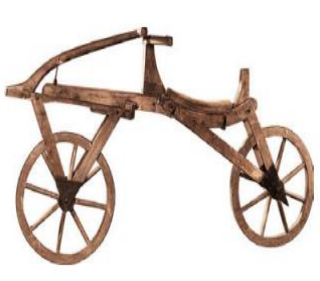
\includegraphics[width=0.6\textwidth]{image2.png}
\caption{Primera bicicleta (Draisiana)}
\label{fig:draisiana}
\end{figure}

\begin{figure}[H]
\centering
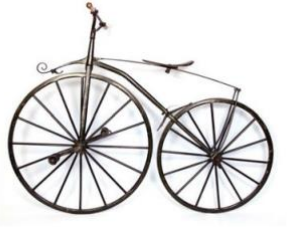
\includegraphics[width=0.6\textwidth]{image3.png}
\caption{Bicicleta Penny Farthing}
\label{fig:pennyfarthing}
\end{figure}

\subsection{Dinámica de la Bicicleta}

La dinámica de montar y equilibrar una bicicleta implica un complejo proceso de control físico y neuromecánico en el que el ciclista mantiene activo el equilibrio del sistema bicicleta-ciclista. Aunque una bicicleta puede mostrar cierta autoestabilidad cuando está en movimiento debido a sus características de diseño, la estabilidad real con un ciclista montado es más difícil de describir matemáticamente, ya que depende de las acciones de control realizadas por el propio ciclista (Cain, 2016).

\subsection{Movimiento Giroscópico}

El giróscopo o giroscopio es un dispositivo mecánico formado esencialmente por un cuerpo con simetría de rotación que gira alrededor de su eje de simetría y cuyo eje de giro no es fijo, sino que puede cambiar de orientación en el espacio. Cuando se somete el giroscopio a un momento de fuerza que tiende a cambiar la orientación del eje de rotación su comportamiento es aparentemente paradójico ya que el eje de rotación, en lugar de cambiar de dirección como lo haría un cuerpo que no girase, cambia de orientación en una dirección perpendicular a la dirección ``intuitiva''.

\begin{figure}[H]
\centering
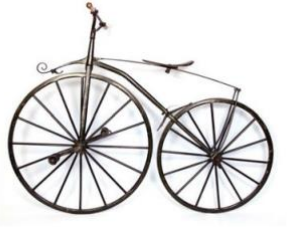
\includegraphics[width=0.7\textwidth]{image3.png}
\caption{Ejemplo de un volante con eje horizontal}
\label{fig:volante_horizontal}
\end{figure}

\subsubsection{Efecto Giroscópico}

El efecto giroscópico es uno de los fenómenos más fascinantes de la física rotacional y es el principio que permite que el proyecto mantenga el equilibrio.

\textbf{Momento Angular ($\mathbf{L}$)}

Cuando un objeto (como el volante de inercia) gira rápidamente alrededor de su eje de simetría, posee una magnitud vectorial llamada momento angular. Su dirección se determina por la regla de la mano derecha: si envuelves el eje con tus dedos en la dirección del giro, tu pulgar apunta en la dirección de $L$.

Ecuación:
\begin{equation}
L = I\omega
\end{equation}

donde $I$ es el momento de inercia y $\omega$ es la velocidad angular.

\textbf{Precesión ($\mathbf{\Omega_p}$)}

Es el movimiento más característico del efecto giroscópico. Si intentas inclinar el eje de un objeto que gira (aplicando un torque $\tau$), el eje no se moverá en la dirección en la que lo empujas, sino en una dirección perpendicular tanto al torque como al momento angular original.

Ecuación de la velocidad de precesión:
\begin{equation}
\Omega_p = \frac{\tau}{L} = \frac{mgr}{I\omega}
\end{equation}

\subsection{Estimación de Orientación mediante Filtros Complementarios}

La estimación precisa del ángulo de inclinación u orientación es fundamental en el control de sistemas dinámicos, como el péndulo invertido. Para lograr esto, se emplean comúnmente sensores inerciales que incluyen acelerómetros y giroscopios. Sin embargo, cada uno de estos sensores presenta limitaciones inherentes que impiden su uso aislado de manera eficiente en sistemas de control de retroalimentación (Adams, s.f.).

\subsubsection{El Acelerómetro y la Medición de Inclinación}

El acelerómetro mide la aceleración debida a la gravedad para determinar la orientación con respecto al centro de la Tierra. En condiciones estáticas, el ángulo de inclinación se puede calcular mediante la relación entre los ejes de aceleración $(a_x, a_y)$:

\begin{equation}
\theta = \arctan\left(\frac{a_y}{a_x}\right)
\end{equation}

\subsubsection{El Giroscopio y la Velocidad Angular}

El giroscopio mide la velocidad de rotación (grados por segundo). Para obtener el ángulo de inclinación, se debe integrar la medición en el tiempo:

\begin{equation}
\theta = \theta_0 + g_z\Delta t
\end{equation}

\subsubsection{Filtro Complementario}

El filtro complementario surge como una solución eficiente y de bajo costo computacional para mitigar las deficiencias de ambos sensores. Su función principal es combinar las señales mediante el uso de un filtro de paso bajo para el acelerómetro y un filtro de paso alto para el giroscopio.

Según Adams (s.f.), el algoritmo combina la estabilidad del acelerómetro a largo plazo con la precisión del giroscopio a corto plazo mediante un promedio ponderado:

\begin{equation}
\text{Ángulo} = W \cdot (\text{Ángulo}_{prev} + \omega \cdot \Delta t) + (1-W) \cdot \text{Ángulo}_{accel}
\end{equation}

Donde $W$ es un peso (típicamente cercano a 0.99) que permite que el sistema ignore el ruido de alta frecuencia del acelerómetro mientras corrige la deriva del giroscopio utilizando la referencia gravitacional.

\subsection{Controlador PID}

De acuerdo con National Instruments (2025), el algoritmo PID es el controlador más utilizado en la industria debido a su robustez y simplicidad. Su funcionamiento se basa en un mecanismo de retroalimentación que calcula continuamente el valor de un ``error'' como la diferencia entre una variable de proceso medida y un punto de consigna deseado. El controlador intenta minimizar este error ajustando las entradas de control del sistema a través de la suma de tres parámetros: el proporcional, que determina la reacción al error actual; el integral, que permite eliminar el error de estado estacionario acumulado; y el derivativo, que actúa como un amortiguador al predecir el comportamiento futuro del error basado en su tasa de cambio.

\subsubsection{La Ecuación General del PID}

En el dominio del tiempo, la señal de control se define mediante la siguiente ecuación:

\begin{equation}
u(t) = K_p e(t) + K_i \int_{0}^{t} e(\tau)d\tau + K_d \frac{de(t)}{dt}
\end{equation}

\subsection{Microcontrolador ESP32}

El ESP32 representa una evolución significativa respecto a arquitecturas anteriores (como el PSoC o Arduino), ofreciendo una infraestructura diseñada para el procesamiento paralelo y el control de precisión.

\subsubsection{Arquitectura Xtensa Dual-Core de 32 bits}

A diferencia de los microcontroladores de un solo núcleo, el ESP32 integra dos núcleos de procesamiento (denominados Protocol CPU y App CPU) que pueden operar de forma independiente hasta a 240 MHz.

\subsubsection{Sensor de Movimiento Integral (MPU9250)}

El MPU9250 es un dispositivo de seguimiento de movimiento de 9 ejes (9-DOF) que combina dos chips en un solo paquete: un acelerómetro y giroscopio de 3 ejes (MPU6500) y un magnetómetro de 3 ejes (AK8963). Esta integración lo convierte en un sistema MARG (Magnetic, Angular Rate, and Gravity), ideal para aplicaciones de navegación y equilibrio (InvenSense, 2016).

\section{Marco Legal}

El desarrollo del presente proyecto de investigación se encuentra enmarcado bajo normatividades nacionales e internacionales que regulan tanto el diseño mecánico como la implementación de sistemas electrónicos de control. A continuación, se detallan las normas que intervienen en la ejecución de la plataforma de estabilización:

\subsection{Normativa de Control y Programación}

\textbf{IEC 61131-3:} Esta norma internacional es el estándar para la programación de controladores industriales. Se aplica a los controladores programables y sus periféricos asociados, tales como herramientas de programación, depuración e interfaces hombre-máquina (HMI).

\subsection{Normativa de Representación Gráfica y Diseño Mecánico}

\textbf{NTC 1580 (Dibujo Técnico. Escalas):} Esta norma establece las escalas y su designación para uso en dibujos técnicos en cualquier rama de la ingeniería.

\textbf{NTC 1832 (Representación Convencional de Engranajes):} Establece las reglas para la representación de la parte dentada de los engranajes.

\textbf{NTC 2529 (Tolerancias Geométricas):} Proporciona las guías para la verificación de tolerancias de forma, orientación, posición y desarrollo.

\subsection{Normativa de Seguridad en Baterías y Sistemas de Potencia}

\textbf{IEC 62133-2:} Es el estándar internacional para celdas y baterías de litio recargables.

\textbf{NTC 2054 (Material de Transporte. Bicicletas):} Define los requisitos de seguridad y métodos de ensayo para bicicletas.

\subsection{Estándares de Ingeniería de Control y Software}

\textbf{IEEE Std 1016-2009:} Proporciona los lineamientos para la documentación de diseño de software.

% ============================================
% CAPÍTULO 7: ACTIVIDADES REALIZADAS
% ============================================
\chapter{Actividades realizadas durante la pasantía}

Presentación del cómo se llevó a cabo la pasantía. Se deben presentar las actividades organizadas por fases en un diagrama de Gantt de acuerdo con la propuesta aprobada. Se debe incluir una descripción y análisis de cada una de las actividades que incluya los métodos, técnicas, estándares y normas empleadas.

\section{Investigación de sistemas similares para la obtención de criterios de diseño}

A partir del estudio de los diferentes proyectos implementados, los cuales se mencionan en el presente documento en el Capítulo 6 (Marco de Referencia), se optó por tomar como base dos modelos de diseño mecánico diferentes. En esta sección se describe el procedimiento y el paso a paso seguido para la implementación de cada uno de estos diseños. La selección del diseño más adecuado se definió de manera progresiva, con base en las pruebas realizadas a lo largo del desarrollo del proyecto, permitiendo identificar aquel que ofrecía mejores condiciones de eficiencia y un comportamiento más estable del sistema.

\subsection{Diseño Del Volante}

Para este diseño en primera instancia se decidió usar una bicicleta tipo carreras la cual tiene como dimensiones las mencionadas en la figura \ref{fig:bici_dimensiones}, tomando en cuenta estas dimensiones, se realiza un análisis y se determina que como primera muestra de datos bajo el comportamiento de la planta se podría adecuar, un soporte vertical en el cual se podría adecuar un motor que en primera instancia se encargó de mover un volante de inercia con un peso aproximado de 2 kilogramos.

\begin{figure}[H]
\centering
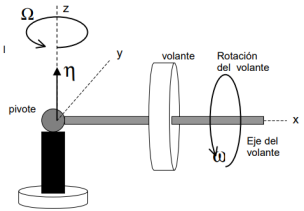
\includegraphics[width=0.7\textwidth]{image4.png}
\caption{Dimensiones de la bicicleta tipo carreras utilizada}
\label{fig:bici_dimensiones}
\end{figure}

\begin{figure}[H]
\centering
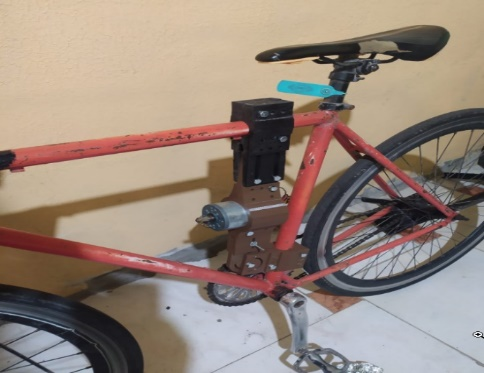
\includegraphics[width=0.7\textwidth]{image5.jpeg}
\caption{Primer diseño del volante de inercia con soporte vertical}
\label{fig:primer_diseno}
\end{figure}

Para este modelo inicial se lograron identificar varias falencias con el modelo, el cual por el peso del volante y las dimensiones de la bicicleta, no contaba con el torque necesario, para realizar el control o la estabilidad deseada en la bicicleta.

Esta primera prueba de la planta fue indispensable ya que se lograron identificar grandes falencias en el modelo, una de las grandes falencias que se identificó que al ubicar el volante de inercia en esta posición, no ayudaba mucho a la estabilidad de la bicicleta ya que su centro de gravedad se veía afectado e interfería con la estabilidad, además que por su diseño el controlador debería ser más robusto y capaz de controlar movimientos bruscos solo con el cambio de sentido de giro del motor.

\section{Análisis del modelo matemático del sistema y Diseño tridimensional (3D)}

A partir de los resultados obtenidos en la primera planta, se optó por construir un segundo modelo el cual su diseño se caracterizó ubicar el volante en la parte superior de la bicicleta, este diseño a diferencia del anterior acoplaba el movimiento de giro del volante a través de un motor DC, el cual solo giraba en un solo sentido.

\begin{figure}[H]
\centering
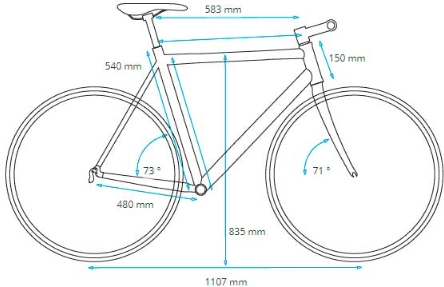
\includegraphics[width=0.7\textwidth]{image6.jpeg}
\caption{Segundo diseño con volante en la parte superior}
\label{fig:segundo_diseno}
\end{figure}

Como se observa en la figura \ref{fig:segundo_diseno}, el motor DC está acoplado directamente al volante de inercia, este a través de su eje. La intención en esta segunda etapa fue verificar el cambio del comportamiento de la estabilidad de la bicicleta, ya que el volante fue remplazado con otro de mayor peso este cuenta con un peso estimado de 10 kilogramos, a diferencia del volante anterior este cuenta con un diseño totalmente diferente y su material es de hierro.

Este nuevo diseño está pensado en que el sistema pueda aprovechar al máximo el momento de inercia, cuyo diseño se compone de un volante tipo anillo, el cual cuenta con un anillo exterior mayor al resto del volante que en su parte interior tiene un anillo de menor grosor en comparación al exterior.

\begin{figure}[H]
\centering
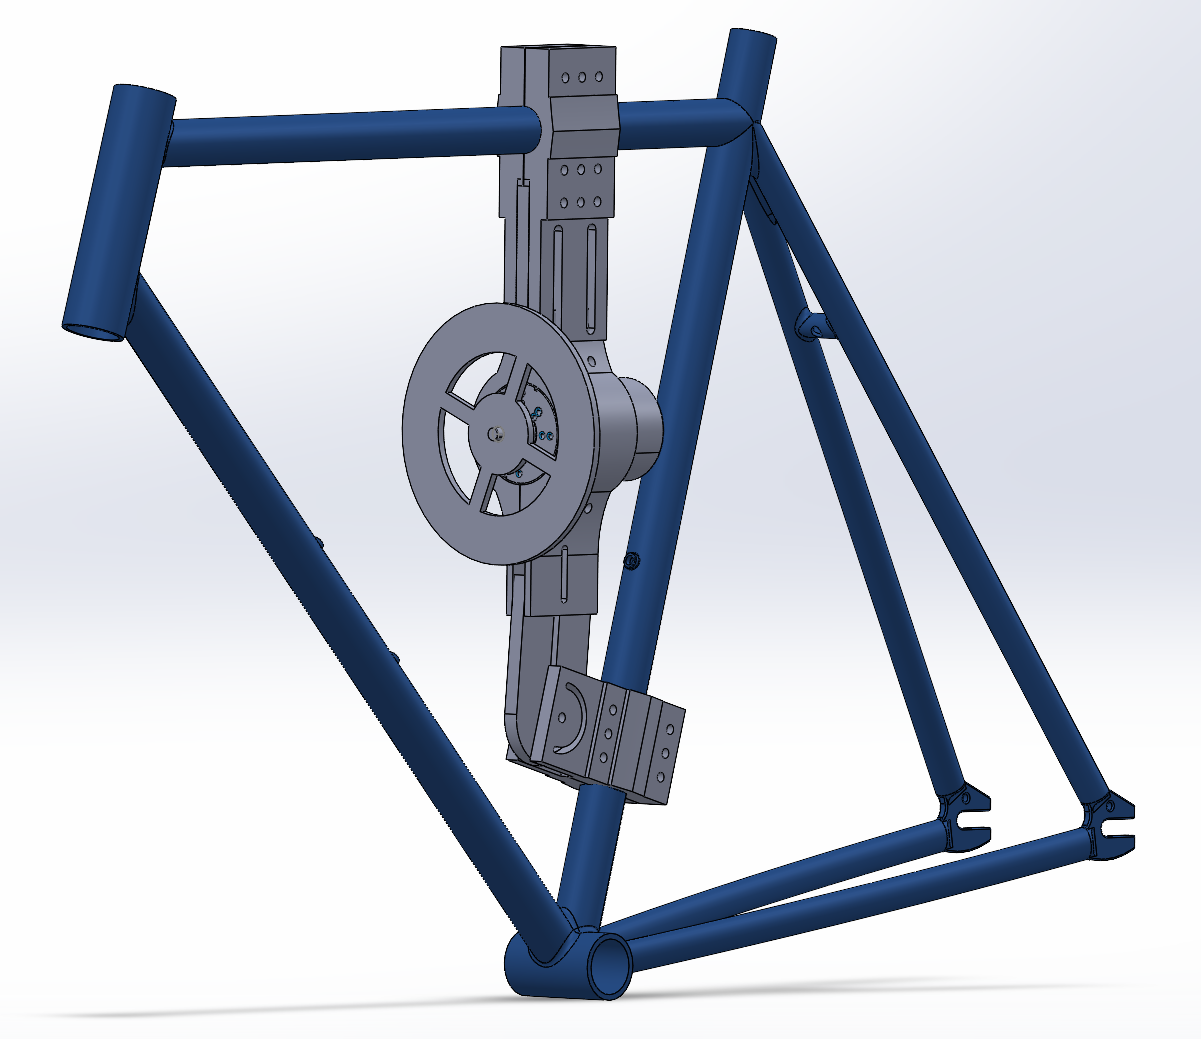
\includegraphics[width=0.6\textwidth]{image7.png}
\caption{Volante de inercia tipo anillo optimizado}
\label{fig:volante_anillo}
\end{figure}

\begin{figure}[H]
\centering
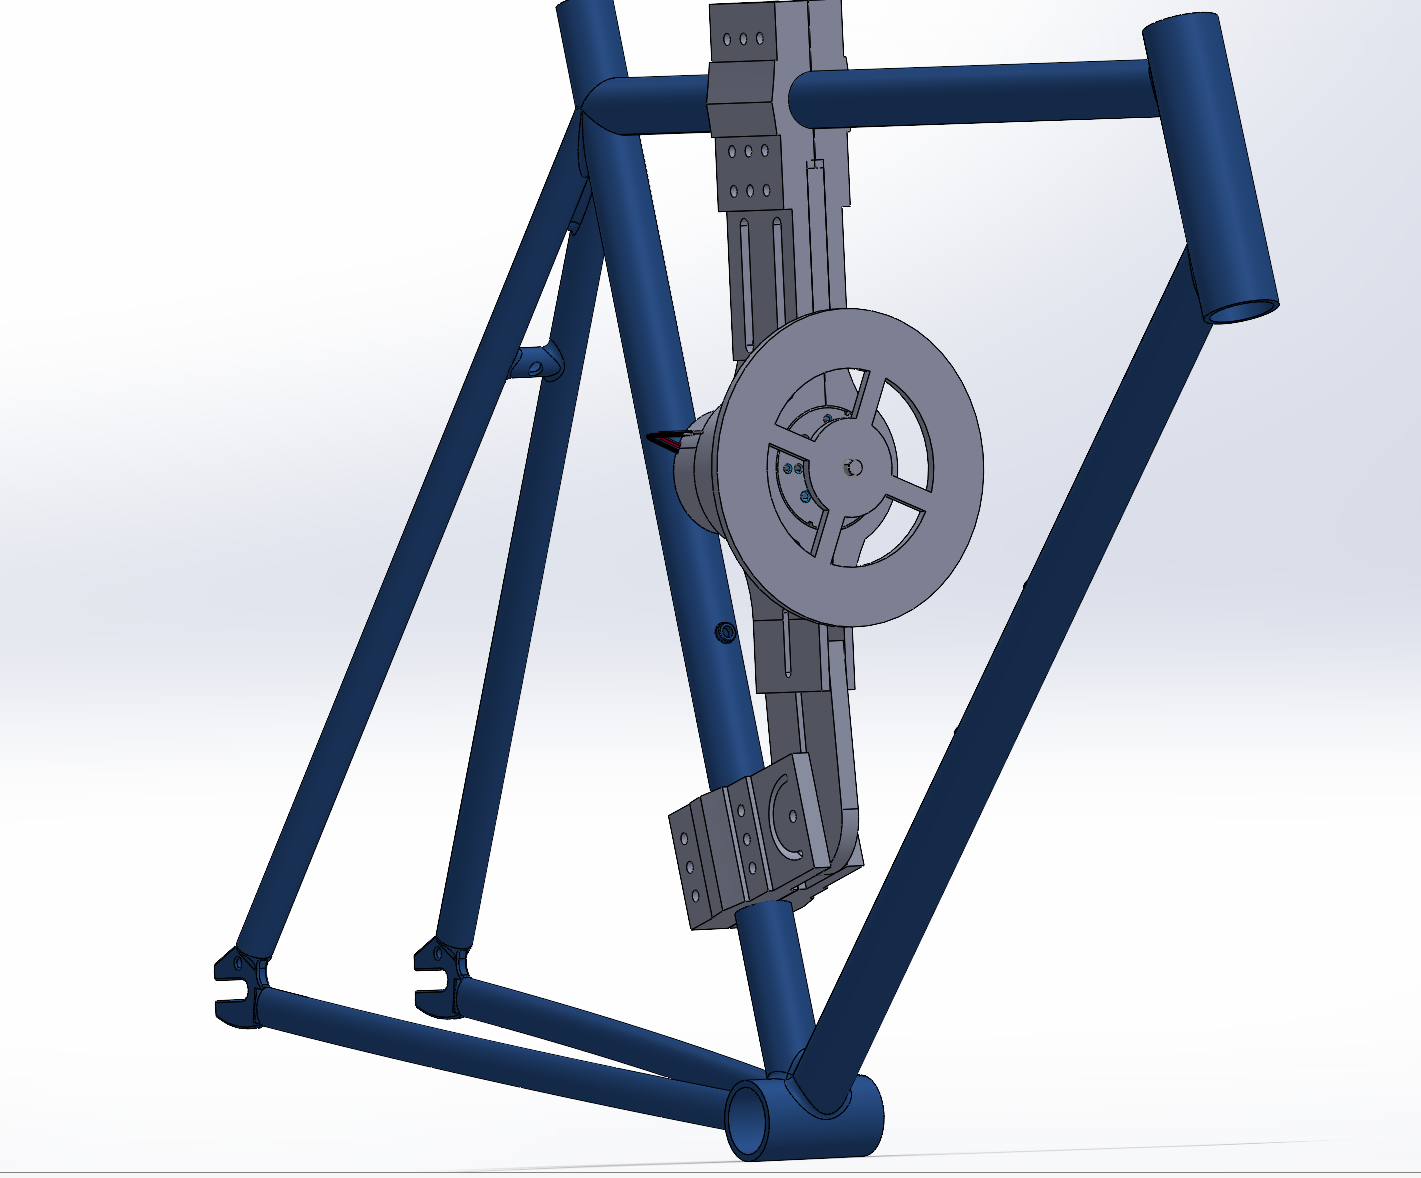
\includegraphics[width=0.7\textwidth]{image8.png}
\caption{Diseño detallado del volante de inercia}
\label{fig:volante_detalle}
\end{figure}

Este diseño permite:
\begin{itemize}
\item \textbf{Mayor Momento Angular:} El momento angular es la cantidad de rotación almacenada y el factor fundamental para la estabilidad, proporcionando mayor resistencia del volante a ser inclinado o perturbado.
\item \textbf{Mayor Torque Giroscópico de Estabilización:} Esto significa que puede contrarrestar fuerzas externas (como un viento lateral o una inclinación rápida) con mayor eficacia, logrando una estabilización más robusta.
\item \textbf{Mayor Almacenamiento de Energía Cinética:} Esto le da al sistema una mayor reserva de energía para mantener la velocidad durante los picos de demanda de torque de corrección.
\end{itemize}

Con este nuevo diseño del volante de inercia es indispensable disponer y calcular el momento de inercia generado por este mismo.

\begin{figure}[H]
\centering
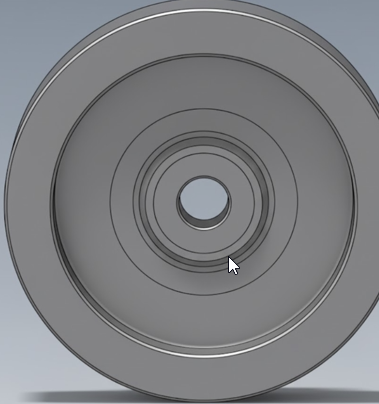
\includegraphics[width=0.75\textwidth]{image9.png}
\caption{Cálculo del momento de inercia del volante - Parte 1}
\label{fig:calculo_inercia1}
\end{figure}

\begin{figure}[H]
\centering
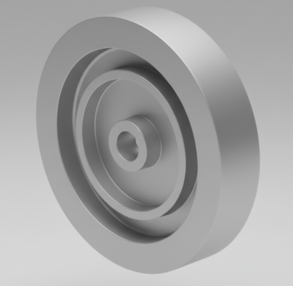
\includegraphics[width=0.75\textwidth]{image10.png}
\caption{Cálculo del momento de inercia del volante - Parte 2}
\label{fig:calculo_inercia2}
\end{figure}

Al realizar los cálculos corroboramos que el nuevo volante de inercia al tener un giro aproximado de 3000 RPM podría suministrar un momento de inercia de 25.36 kgm²/s, este parámetro es super indispensable, ya se depende de él, directamente para aplicar el giro de la estructura de donde está aplicado para aplicar la precesión giroscópica y realizar el control de esta directamente.

\section{Mecanizado y ensamble de la planta física}

En esta segunda etapa se realizó un diseño mecánico el cual permite acoplar directamente la bicicleta a la estructura que asegura el volante y motor. En esta etapa la estructura inicialmente se instala en la parte superior de la bicicleta, adicionalmente la estructura acopla directamente el motor de tracción del volante.

\begin{figure}[H]
\centering
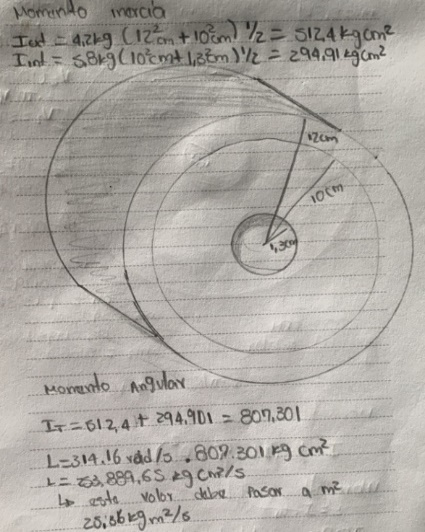
\includegraphics[width=0.7\textwidth]{image11.jpeg}
\caption{Estructura de soporte del motor y volante instalada en la bicicleta}
\label{fig:estructura_instalada}
\end{figure}

\begin{figure}[H]
\centering
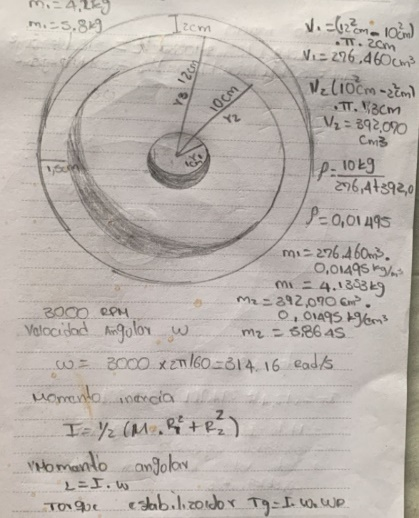
\includegraphics[width=0.7\textwidth]{image12.jpeg}
\caption{Vista detallada del acople del motor al volante}
\label{fig:acople_motor}
\end{figure}

Por otra parte esta estructura es la que directamente se encargó de realizar el movimiento de todo el conjunto, esto se logró a través de un eje de dirección vertical con rodamientos, tipo chumacera, este instalado directamente sobre el marco de la bicicleta.

\begin{figure}[H]
\centering
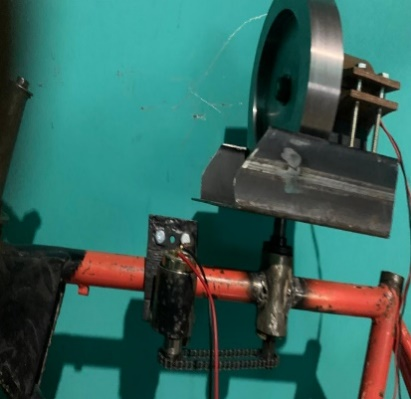
\includegraphics[width=0.6\textwidth]{image13.jpeg}
\caption{Sistema de eje vertical con rodamientos tipo chumacera}
\label{fig:eje_vertical}
\end{figure}

Para esta etapa también fue incluido un motor reductor, el cual cumple como función principal controlar la dirección de la estructura motor-volante, este cambia el sentido de giro de la estructura a través de un piñón ubicado en el eje del motor de control y otro en el eje de dirección instalado, estos dos se comunican entre sí por medio de una cadena, que transmite el movimiento del motor reductor al eje de dirección.

\begin{figure}[H]
\centering
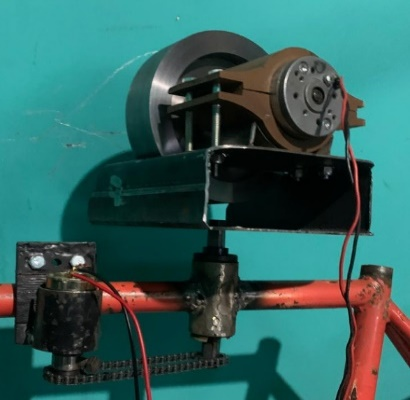
\includegraphics[width=0.7\textwidth]{image14.jpeg}
\caption{Sistema de piñón y cadena para control de dirección}
\label{fig:pinon_cadena}
\end{figure}

En esta etapa del proyecto se realizan varias modificaciones significativas ya que el mecanismo implementado para la dirección, carecía de las condiciones necesarias para poder ejercer el movimiento a todo el conjunto, a partir de ello se realizó el cambio del mecanismo por un mecanismo tipo polea en el cual se realizó el cambio de los piñones y se remplazó la cadena por una correa de arrastre.

\begin{figure}[H]
\centering
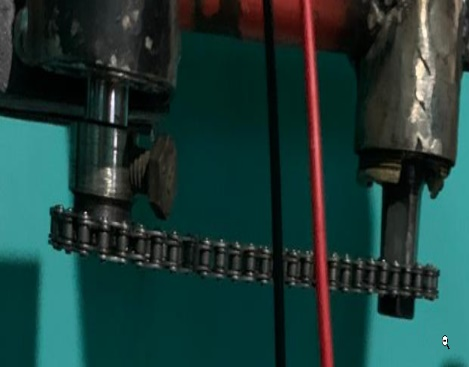
\includegraphics[width=0.7\textwidth]{image15.jpeg}
\caption{Mecanismo tipo polea con correa de arrastre}
\label{fig:polea_correa}
\end{figure}

\subsection{Control sistema de dirección}

A partir de esta, comenzaron los primeros pasos para controlar la dirección de la estructura motor-volante, para ello se realizó un control de dirección del motor por medio de un controlador PSoC y un driver BTS7960.

\begin{figure}[H]
\centering
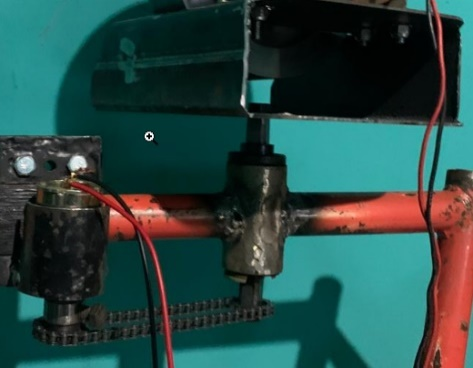
\includegraphics[width=0.75\textwidth]{image16.jpeg}
\caption{Controlador PSoC y driver BTS7960 para control del motor}
\label{fig:psoc_driver}
\end{figure}

Para esta etapa inicialmente se realizaron pruebas para verificar el funcionamiento del control de giro cuando el volante estaba en movimiento. Se evidenció una carencia de agarre en el sistema piñón-correa. El peso y la fuerza ejercida por la estructura resultaron ser superiores a la capacidad de arrastre de la polea y la correa acopladas al motor.

\begin{figure}[H]
\centering
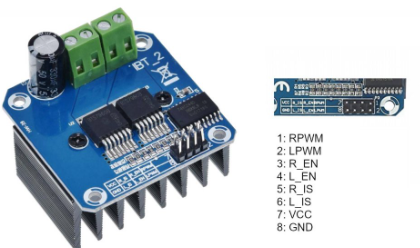
\includegraphics[width=0.7\textwidth]{image17.png}
\caption{Problemas identificados en el sistema de transmisión}
\label{fig:problemas_transmision}
\end{figure}

En este diseño se realizaron cambios tanto en la estructura de soporte motor como en la versión de la bicicleta, para esta versión de la bicicleta se redujo el tamaño para lograr establecer la planta más estable, su diseño acopla una estructura de base motor más reducida y más liviana.

\begin{figure}[H]
\centering
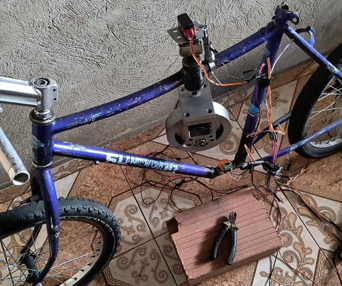
\includegraphics[width=0.7\textwidth]{image18.png}
\caption{Bicicleta de tamaño reducido con nueva estructura}
\label{fig:bici_reducida}
\end{figure}

Por otra parte el diseño redujo pérdidas de energía en la transmisión de potencia, ya que en esta etapa se remplazó el sistema de polea y el motor reductor por un servomotor que se acopla directamente al eje vertical.

\begin{figure}[H]
\centering
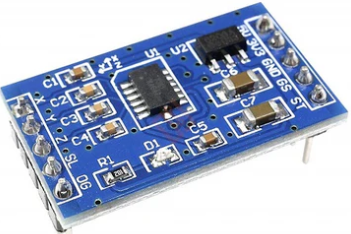
\includegraphics[width=0.6\textwidth]{image19.png}
\caption{Servomotor acoplado directamente al eje vertical}
\label{fig:servomotor_eje}
\end{figure}

A continuación se logró poner a prueba el cambio de giro del motor de una manera más eficiente y con ello continuar con la siguiente etapa del proyecto la cual constaba en sensar la posición exacta de la bicicleta.

\section{Implementación del sistema de comunicación}

\subsection{Sensado de la posición de la bicicleta}

Para verificar la posición de la bicicleta se pusieron a prueba dos sensores tipo acelerómetro:

\subsubsection{MMA7361}

Inicialmente, se incorporó a la planta el sensor MMA7361, con el cual se realizaron las primeras mediciones de la inclinación en el eje Z. No obstante, durante la etapa de pruebas se determinó que el sensor analógico presentaba una alta susceptibilidad al ruido.

\begin{figure}[H]
\centering
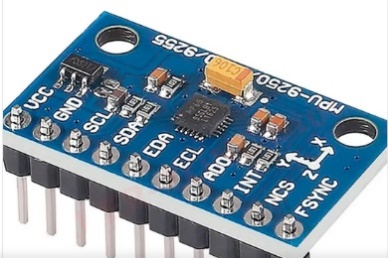
\includegraphics[width=0.6\textwidth]{image20.jpeg}
\caption{Sensor analógico MMA7361}
\label{fig:mma7361}
\end{figure}

Como primera estrategia para mitigar este problema, se implementaron filtros digitales con el objetivo de atenuar las señales parásitas y permitir que el sistema trabajara únicamente con la señal útil proven Wendy del sensor.

\begin{figure}[H]
\centering
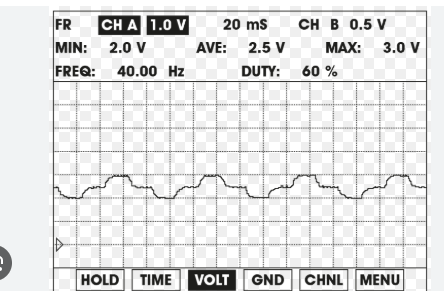
\includegraphics[width=0.75\textwidth]{image21.png}
\caption{Señal del MMA7361 sin filtro - con ruido}
\label{fig:mma7361_sin_filtro}
\end{figure}

A pesar de esta mejora, el sistema continuó presentando un comportamiento inestable durante su operación. Tras realizar un análisis más detallado del sistema y llevar a cabo nuevas pruebas experimentales, se concluyó que la principal fuente del problema era el uso de un sensor analógico.

\subsubsection{MPU9250}

Para esta etapa del proyecto se implementó el sensor digital MPU9250, el cual integra un acelerómetro y un giroscopio en los tres ejes (x,y,z), permitiendo la medición de aceleraciones lineales y velocidades angulares en los tres ejes.

\begin{figure}[H]
\centering
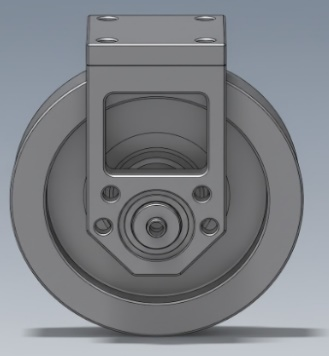
\includegraphics[width=0.6\textwidth]{image22.jpeg}
\caption{Sensor digital MPU9250}
\label{fig:mpu9250}
\end{figure}

\begin{figure}[H]
\centering
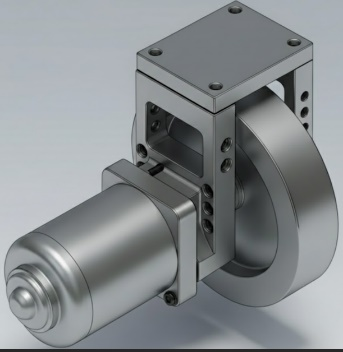
\includegraphics[width=0.7\textwidth]{image23.jpeg}
\caption{MPU9250 montado en la planta}
\label{fig:mpu9250_montado}
\end{figure}

El MPU9250 y el microcontrolador realizan e intercambian información mediante el protocolo I²C, lo cual permite una transmisión digital de los datos, reduciendo significativamente la susceptibilidad al ruido eléctrico en comparación con el sensor MMA7361.

\begin{figure}[H]
\centering
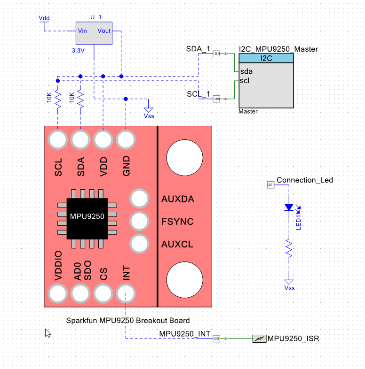
\includegraphics[width=0.75\textwidth]{image24.png}
\caption{Comparación de señales MMA7361 vs MPU9250 - sin filtro}
\label{fig:comparacion_sensores1}
\end{figure}

\begin{figure}[H]
\centering
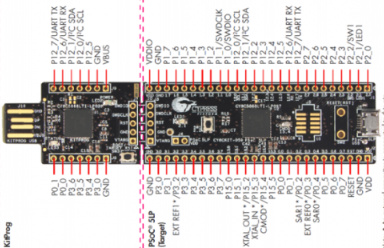
\includegraphics[width=0.75\textwidth]{image25.png}
\caption{Comparación de señales MMA7361 vs MPU9250 - con filtro}
\label{fig:comparacion_sensores2}
\end{figure}

\begin{figure}[H]
\centering
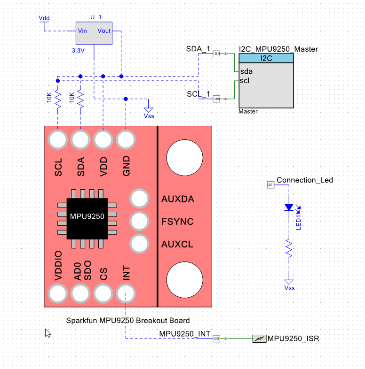
\includegraphics[width=0.75\textwidth]{image26.png}
\caption{Señal filtrada del MPU9250 mostrando mejor calidad}
\label{fig:mpu9250_filtrada}
\end{figure}

\begin{figure}[H]
\centering
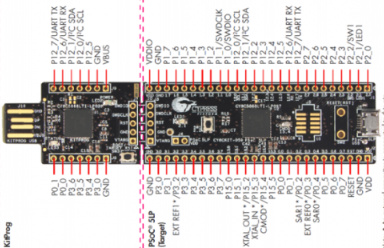
\includegraphics[width=0.75\textwidth]{image27.png}
\caption{Detalle de la reducción de ruido después del filtrado}
\label{fig:reduccion_ruido}
\end{figure}

A partir del análisis anterior y como revelan las gráficas de la señal de ángulo, la calidad de la señal emitida por el sensor digital es mucho más limpia y presenta una mejor condición para que el microcontrolador pueda interpretarla de una mejor manera.

\section{Implementación del sistema de control}

Con base en los resultados obtenidos anteriormente, y ante la necesidad de implementar un sistema de control eficiente, se determinó en una primera instancia realizar diversas modificaciones en la planta física.

\subsection{Modificaciones estructurales}

Se llevó a cabo un análisis estructural de carácter experimental y de observación, basado en la inspección visual del sistema durante su operación, así como en la evaluación del comportamiento dinámico de la planta ante diferentes condiciones de funcionamiento.

A partir de la identificación de los puntos críticos, se procedió a realizar modificaciones en la estructura mecánica utilizando el software de diseño SolidWorks.

\begin{figure}[H]
\centering
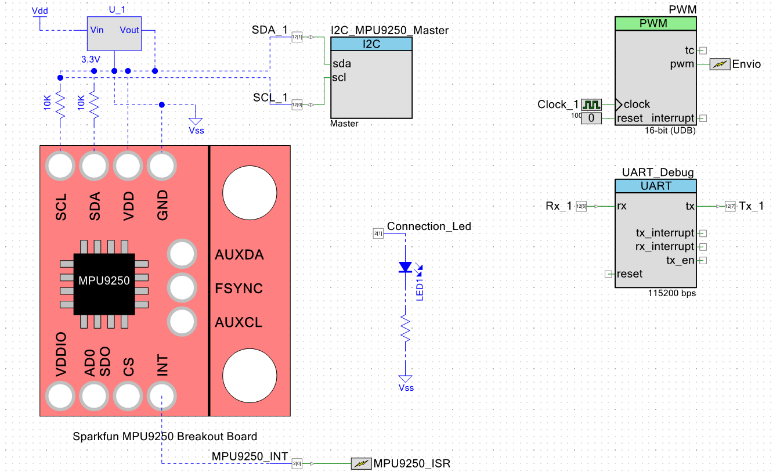
\includegraphics[width=0.75\textwidth]{image28.png}
\caption{Diseño en SolidWorks de la nueva estructura optimizada}
\label{fig:solidworks_estructura}
\end{figure}

\begin{figure}[H]
\centering
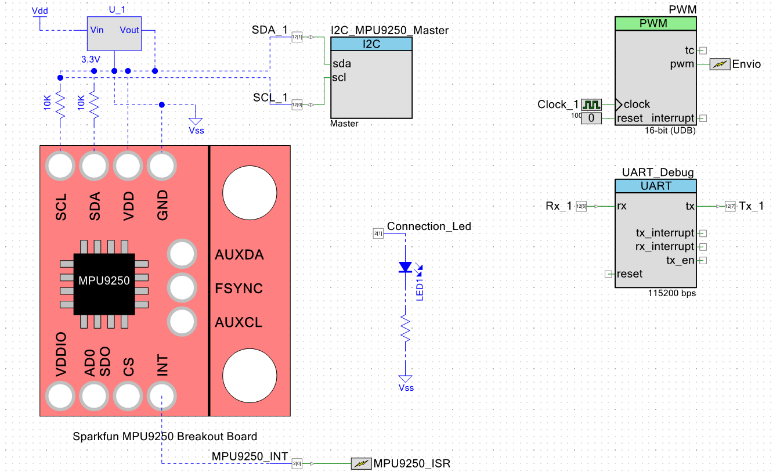
\includegraphics[width=0.75\textwidth]{image29.png}
\caption{Vista isométrica del nuevo diseño estructural}
\label{fig:estructura_isometrica}
\end{figure}

En la figura \ref{fig:estructura_mejorada} se presentan los resultados del nuevo diseño estructural, en el cual se observa que el soporte del conjunto motor–volante se vuelve más compacto y ligero. Este diseño incorpora tres soportes estructurales que se anclan entre sí mediante múltiples puntos de fijación, conformando una estructura más robusta y rígida.

\begin{figure}[H]
\centering
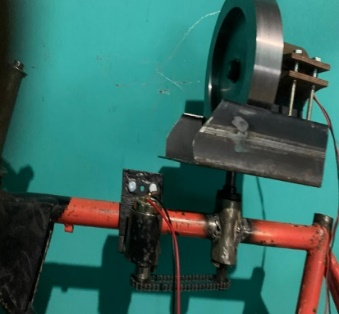
\includegraphics[width=0.7\textwidth]{image30.jpeg}
\caption{Estructura mejorada más compacta y robusta}
\label{fig:estructura_mejorada}
\end{figure}

\begin{figure}[H]
\centering
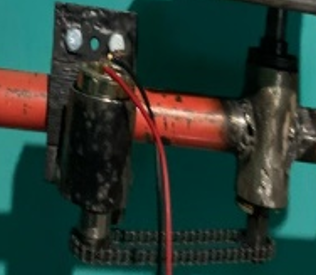
\includegraphics[width=0.7\textwidth]{image31.png}
\caption{Detalle de los soportes estructurales y puntos de anclaje}
\label{fig:soportes_detalle}
\end{figure}

\begin{figure}[H]
\centering
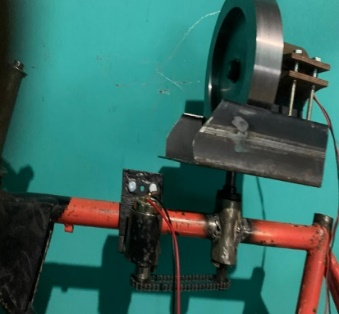
\includegraphics[width=0.7\textwidth]{image32.jpeg}
\caption{Eje solidario del volante con sistema de cuña}
\label{fig:eje_solidario}
\end{figure}

\subsection{Adquisición de datos y tratamiento de la señal}

Dado que el MPU9250 transmite la información mediante el protocolo de comunicación I²C, fue necesario incorporar en la programación del microcontrolador el correspondiente bloque de comunicación I²C.

\begin{figure}[H]
\centering
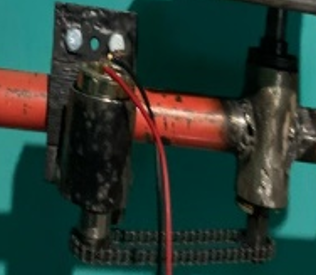
\includegraphics[width=0.8\textwidth]{image33.png}
\caption{Diagrama de bloques de comunicación I²C en PSoC}
\label{fig:i2c_psoc}
\end{figure}

\begin{figure}[H]
\centering
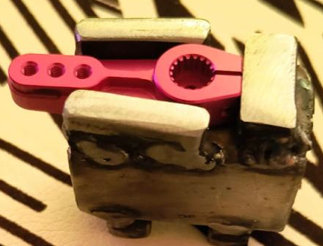
\includegraphics[width=0.7\textwidth]{image34.png}
\caption{Configuración del bloque I²C para el MPU9250}
\label{fig:config_i2c}
\end{figure}

Adicionalmente, con el propósito de visualizar y analizar los datos adquiridos, se implementó un bloque de comunicación RS-232, mediante el cual se enviaban los valores de inclinación al computador.

\begin{figure}[H]
\centering
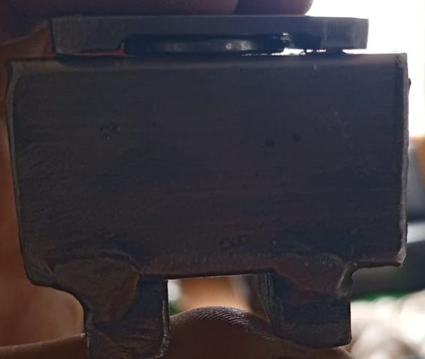
\includegraphics[width=0.8\textwidth]{image35.png}
\caption{Diagrama de bloques de comunicación RS-232}
\label{fig:rs232}
\end{figure}

\begin{figure}[H]
\centering
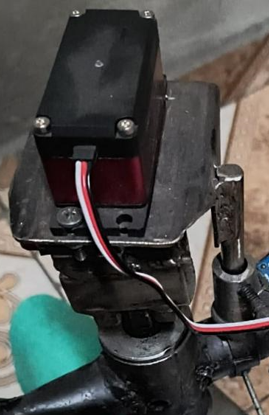
\includegraphics[width=0.75\textwidth]{image36.png}
\caption{Visualización de datos del sensor en el computador}
\label{fig:visualizacion_datos}
\end{figure}

Una vez verificada la correcta adquisición e interpretación de la señal del sensor, los valores fueron utilizados para el cálculo de las señales de salida destinadas al actuador del sistema.

\begin{figure}[H]
\centering
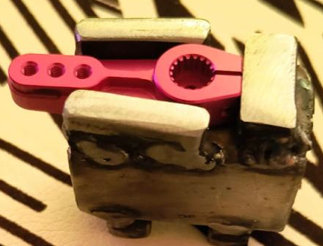
\includegraphics[width=0.8\textwidth]{image37.png}
\caption{Bloque PWM de salida del microcontrolador}
\label{fig:pwm_salida}
\end{figure}

\subsection{Sistema de dirección y actuador}

En contraste a las limitaciones evidenciadas, se determinó la necesidad de reemplazar el motor reductor por un servomotor, el cual ofrecía una mejor respuesta dinámica, mayor precisión en el control de posición y una integración más adecuada con el sistema de control implementado.

Para lograr implementar el servomotor, fue necesario diseñar un soporte para el servomotor, en forma de L con un ajuste de distancia con respecto al marco de la bicicleta.

\begin{figure}[H]
\centering
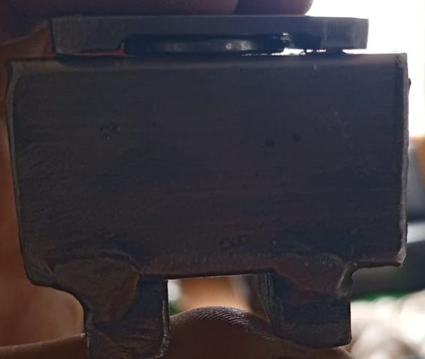
\includegraphics[width=0.7\textwidth]{image38.png}
\caption{Diseño del soporte en L para el servomotor}
\label{fig:soporte_servo1}
\end{figure}

\begin{figure}[H]
\centering
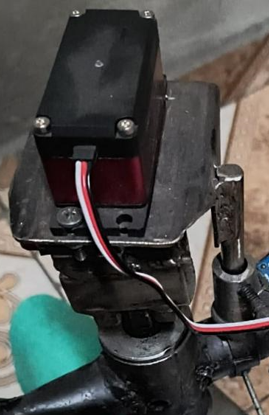
\includegraphics[width=0.7\textwidth]{image39.png}
\caption{Vista detallada del acople del servomotor al eje}
\label{fig:acople_servo}
\end{figure}

\begin{figure}[H]
\centering
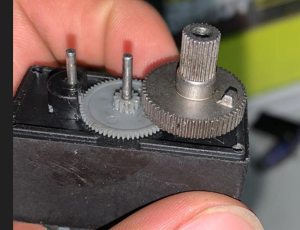
\includegraphics[width=0.7\textwidth]{image40.png}
\caption{Sistema de dirección completo con servomotor instalado}
\label{fig:sistema_direccion}
\end{figure}

\begin{figure}[H]
\centering
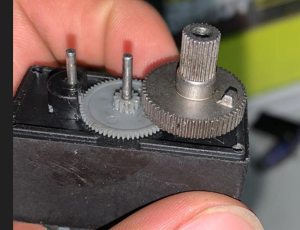
\includegraphics[width=0.6\textwidth]{image41.png}
\caption{Componentes del sistema de dirección}
\label{fig:componentes_direccion}
\end{figure}

Inicialmente se implementó un servomotor con un ángulo de giro de 270° y una capacidad de carga aproximada de 10 kg.

\begin{figure}[H]
\centering
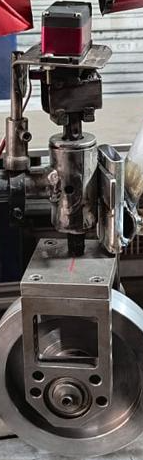
\includegraphics[width=0.6\textwidth]{image42.png}
\caption{Servomotor de 10 kg instalado}
\label{fig:servo_10kg}
\end{figure}

No obstante, durante las pruebas realizadas con la señal de salida generada por el microcontrolador, se evidenció un desgaste prematuro en el sistema interno de engranajes del servomotor.

\begin{figure}[H]
\centering
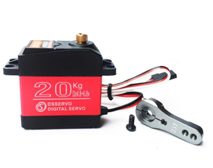
\includegraphics[width=0.7\textwidth]{image43.png}
\caption{Desgaste evidenciado en el servomotor}
\label{fig:desgaste_servo}
\end{figure}

\begin{figure}[H]
\centering
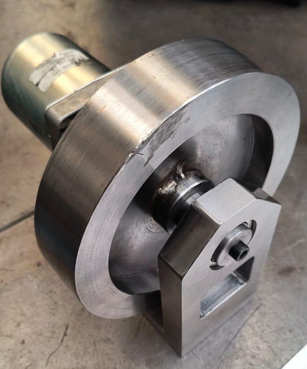
\includegraphics[width=0.6\textwidth]{image44.png}
\caption{Comparación del servomotor antes y después del desgaste}
\label{fig:comparacion_desgaste}
\end{figure}

Como consecuencia, se decidió aumentar la capacidad de carga del actuador, reemplazando el servomotor inicial por un servomotor con una capacidad de carga de 20 kg (modelo DS5180).

\begin{figure}[H]
\centering
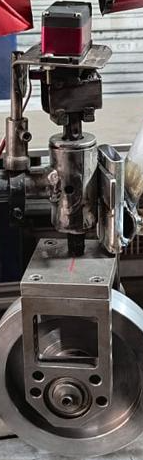
\includegraphics[width=0.6\textwidth]{image45.png}
\caption{Servomotor DS5180 de 20 kg - engranajes metálicos}
\label{fig:servo_20kg}
\end{figure}

\begin{figure}[H]
\centering
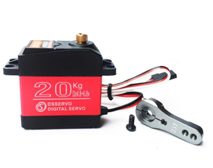
\includegraphics[width=0.7\textwidth]{image46.png}
\caption{Servomotor de 80 kg-cm instalado en la planta final}
\label{fig:servo_80kg}
\end{figure}

\begin{figure}[H]
\centering
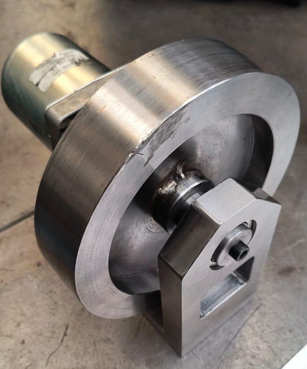
\includegraphics[width=0.7\textwidth]{image47.png}
\caption{Diseño final del sistema de dirección}
\label{fig:diseno_final_direccion}
\end{figure}

\subsection{Integración de los componentes electrónicos en la planta}

Una vez alcanzados los objetivos de diseño y confort de la planta, se procedió al montaje de todos los componentes electrónicos del sistema.

\begin{figure}[H]
\centering
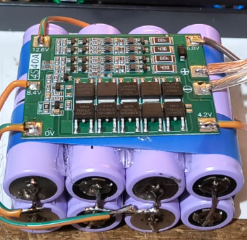
\includegraphics[width=0.7\textwidth]{image48.png}
\caption{Platina de soporte para componentes electrónicos}
\label{fig:platina_electronica}
\end{figure}

\begin{figure}[H]
\centering
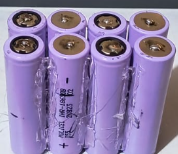
\includegraphics[width=0.7\textwidth]{image49.png}
\caption{Microcontrolador ESP32 y componentes montados}
\label{fig:esp32_montado}
\end{figure}

\subsection{Diseño del sistema de baterías de alimentación}

El  sistema de baterías fue diseñado utilizando celdas de fosfato de hierro-litio (LiFePO₄), cada una con un voltaje nominal aproximado de 3,2 V. Para este diseño, se conectaron seis celdas en serie, obteniendo un voltaje total cercano a 20 V.

\begin{figure}[H]
\centering
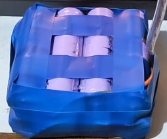
\includegraphics[width=0.6\textwidth]{image50.png}
\caption{Pack de baterías LiFePO₄ de 6 celdas en serie}
\label{fig:pack_baterias}
\end{figure}

\begin{figure}[H]
\centering
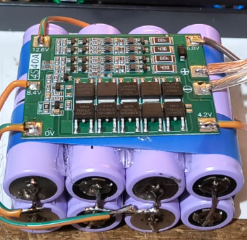
\includegraphics[width=0.7\textwidth]{image51.png}
\caption{Celdas LiFePO₄ individuales de 3.2V}
\label{fig:celdas_lifepo4}
\end{figure}

\begin{figure}[H]
\centering
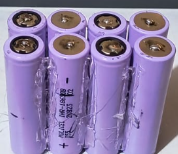
\includegraphics[width=0.7\textwidth]{image52.png}
\caption{Configuración del pack de baterías}
\label{fig:config_baterias}
\end{figure}

\begin{figure}[H]
\centering
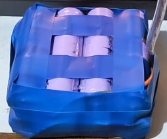
\includegraphics[width=0.6\textwidth]{image53.png}
\caption{Sistema BMS (Battery Management System)}
\label{fig:bms}
\end{figure}

Además, el conjunto de baterías incorpora un sistema de gestión de baterías (BMS), el cual permite supervisar y proteger cada celda de manera individual, garantizando un proceso de carga balanceada y segura.

\begin{figure}[H]
\centering
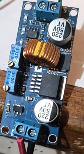
\includegraphics[width=0.7\textwidth]{image54.png}
\caption{Convertidores DC-DC para regulación de voltaje}
\label{fig:dcdc_convertidores}
\end{figure}

\begin{figure}[H]
\centering
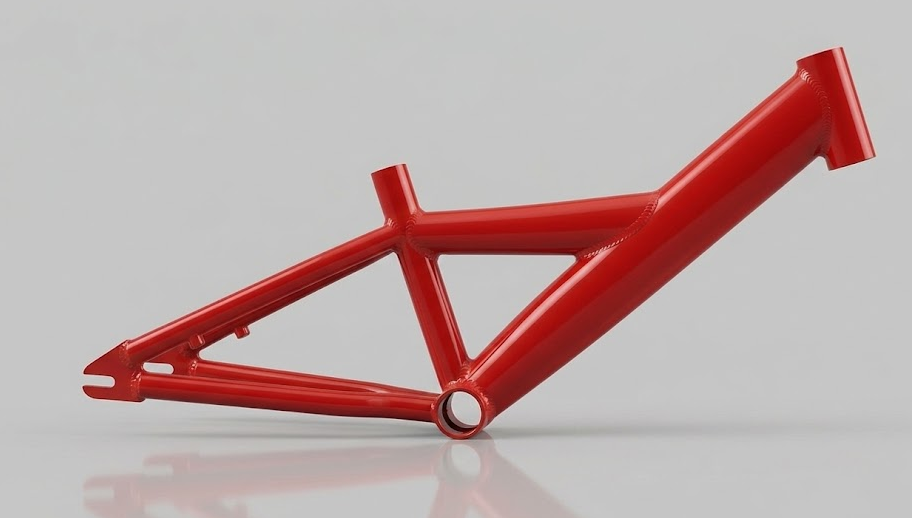
\includegraphics[width=0.7\textwidth]{image55.png}
\caption{Sistema de alimentación completo instalado en la bicicleta}
\label{fig:sistema_alimentacion}
\end{figure}

\subsection{Implementación del control PID y verificación de la señal}

En consecuencia, se iniciaron diferentes pruebas en el circuito de control, lo que condujo a la implementación de un controlador (PID), cuyo objetivo principal fue mejorar la estabilidad del sistema y ampliar el alcance funcional del proyecto.

\begin{figure}[H]
\centering
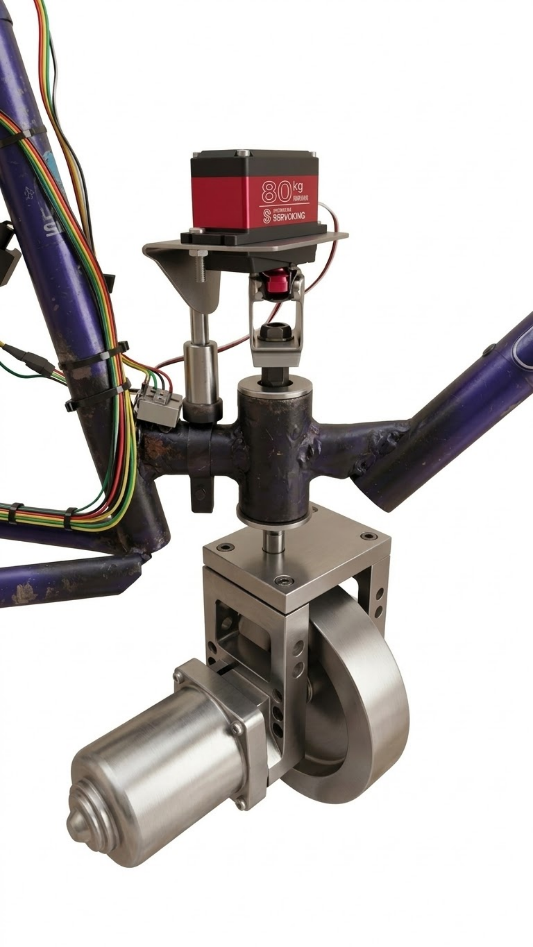
\includegraphics[width=0.8\textwidth]{image56.png}
\caption{Diagrama del sistema de control PID implementado}
\label{fig:diagrama_pid}
\end{figure}

La salida del controlador, generada en forma de una señal PWM, fue inyectada directamente a la entrada de control del servomotor. Dentro del control se tomó como referencia una posición de 140° del motor, definida como el punto medio del rango de operación del sistema de dirección.

\begin{figure}[H]
\centering
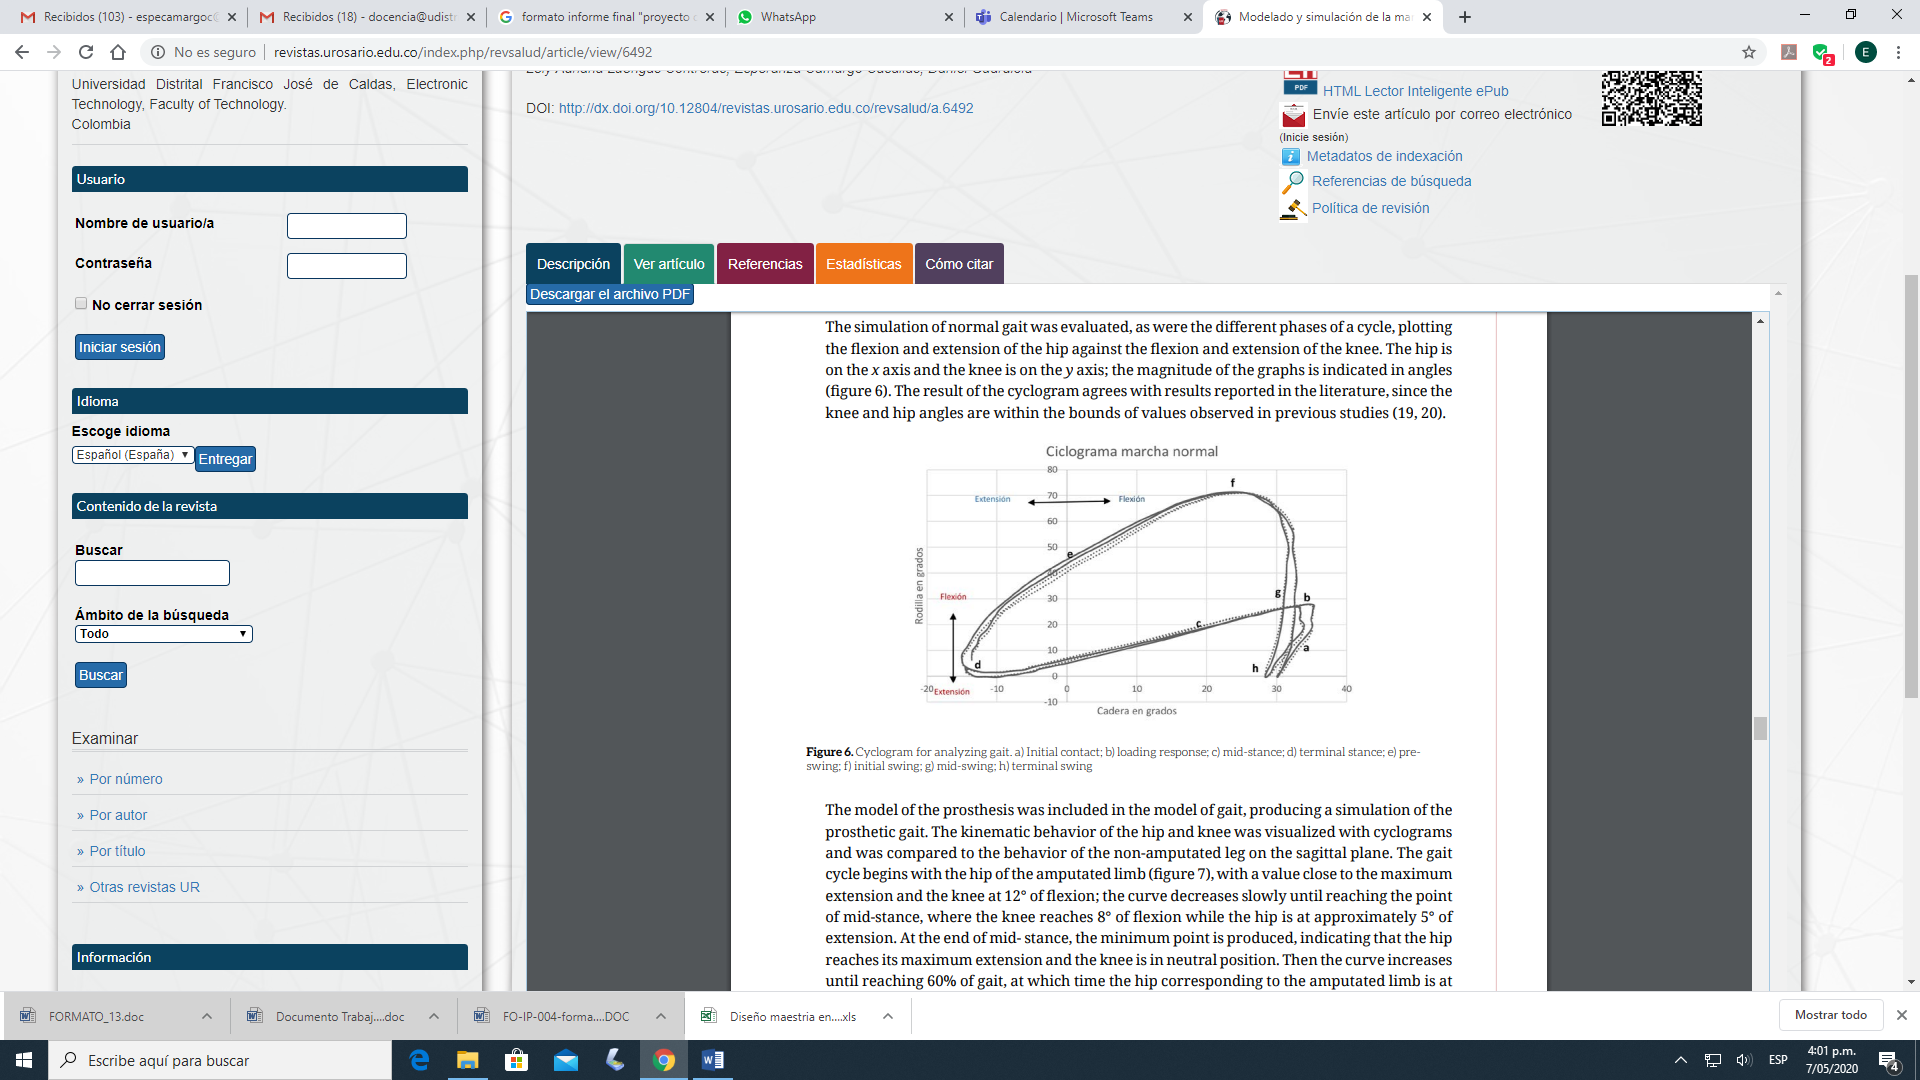
\includegraphics[width=0.8\textwidth]{image57.png}
\caption{Respuesta del sistema con control PID - gráfica de estabilización}
\label{fig:respuesta_pid}
\end{figure}

Al obtener los primeros resultados con el controlador PID, se logró una mejora significativa en la estabilidad de la planta, permitiendo mantener el ángulo de inclinación cercano a 0° durante periodos prolongados. El sistema de control demostró capacidad para rechazar perturbaciones externas y mantener el equilibrio dinámico de la bicicleta.

% ============================================
% CAPÍTULO 8: RESULTADOS
% ============================================
\chapter{Resultados}

El desarrollo del proyecto se ejecutó de manera secuencial mediante cuatro fases fundamentales, integrando la ingeniería mecánica con la electrónica de potencia y control.

\section{Fase 1: Diseño y Construcción Mecánica de la Planta}

Como resultado de la primera fase, se logró una planta mecánica eficiente mediante las siguientes intervenciones:

\begin{itemize}
    \setlength\itemsep{6pt}
    \item \textbf{Reducción de Inercia Estructural:} Se seleccionó y adaptó un marco de bajo peso con el objetivo de minimizar la inercia total del sistema.
    \item \textbf{Centralización del Centro de Masa (CoM):} Se modificó la geometría central del marco para alojar el volante de inercia en la parte inferior-central.
    \item \textbf{Sistemas de Protección y Seguridad:} Se implementaron ruedas auxiliares en el eje trasero.
    \item \textbf{Acondicionamiento para Electrónica:} Se retiró el sillín original para integrar una plataforma de soporte personalizada.
\end{itemize}

\subsection{Diseño del volante de inercia}

El diseño del volante de inercia se centró en optimizar la distribución de masa para maximizar el efecto giroscópico:

\begin{itemize}
    \setlength\itemsep{6pt}
    \item \textbf{Optimización de la Distribución de Masa:} Se diseñó un volante con geometría tipo anillo.
    \item \textbf{Proceso de Fabricación y Ajuste Mecánico:} Partiendo de un bloque sólido de acero, se utilizó un proceso de torneado de precisión.
    \item \textbf{Soporte y Alineación Estructural:} El eje del volante está soportado por dos piezas de acero mecanizadas a medida.
\end{itemize}

\subsection{Sistema de dirección vertical}

Para permitir que el volante de inercia genere el par de torsión necesario para equilibrar la bicicleta, se diseñó un sistema de dirección vertical basado en el principio de precesión giroscópica.

\section{Fase 2: Instrumentación y Procesamiento de Señales}

Una vez consolidada la estructura mecánica, se procedió a la implementación del sistema de percepción.

\subsection{Implementación de la Unidad de Medición Inercial (IMU)}

Para la captura del ángulo de inclinación se utilizó la IMU MPU9250, un dispositivo que integra acelerómetro, magnetómetro y giroscopio.

\subsection{Estrategia de Fusión de Datos: Filtro Complementario}

Debido a las propiedades físicas de cada sensor, se implementó un algoritmo de fusión de datos que permite obtener una medida más precisa que si se usaran de forma aislada.

\subsection{Montaje e Integración del Microcontrolador}

Para la gestión de procesos y el control de la planta, se integró un microcontrolador ESP32 montado sobre una base central diseñada para aislar los componentes electrónicos de las vibraciones mecánicas.

\subsection{Interfaz de Actuación y Acople de Potencia}

La interfaz de actuación constituye el vínculo físico entre las decisiones del microcontrolador y la respuesta dinámica de la planta.

\section{Fase 3: Construcción y Sintonización del Controlador PID}

Esta fase consistió en el desarrollo del algoritmo que permite el equilibrio autónomo:

\begin{itemize}
    \setlength\itemsep{6pt}
    \item Fusión de Sensores
    \item Cálculo del Error
    \item Sintonización de Constantes
\end{itemize}

\section{Fase 4: Adaptación y Construcción del Sistema de Alimentación}

Para garantizar la portabilidad (operación unplugged), se desarrolló un sistema de energía independiente:

\begin{itemize}
    \setlength\itemsep{6pt}
    \item Ensamblaje del Pack LiFePO4
    \item Gestión de Carga (BMS)
    \item Regulación de Voltaje
\end{itemize}

% ============================================
% CAPÍTULO 9: CONCLUSIONES Y RECOMENDACIONES
% ============================================
\chapter{Conclusiones y Recomendaciones}

Esta sección se nutre de las implicaciones de la pasantía en la práctica, de las lecciones metodológicas aprendidas, de las limitaciones de la pasantía, de los aspectos no resueltos y nuevas preguntas o necesidades creadas a partir del mismo, propuestas de nuevos proyectos a partir de los resultados actuales.

% ============================================
% CAPÍTULO 10: REFERENCIAS
% ============================================
\chapter{Referencias}

\section*{Referencias de libros}

Young, H. D., \& Freedman, R. A. (2018). \textit{Física universitaria con física moderna} (14.ª ed.). Pearson Educación.

Serway, R. A., \& Jewett, J. W. (2015). \textit{Física para ciencias e ingeniería} (9.ª ed.). Cengage Learning.

\section*{Referencias de páginas web}

Cain, S. (2016). The mysterious biomechanics of riding – and balancing – a bicycle. University of Michigan Mechanical Engineering. Recuperado de https://me.engin.umich.edu/news-events/news/mysterious-biomechanics-riding-and-balancing-bicycle/

Adams, V. H. (s.f.). Complementary filters. Van Hunter Adams - Cornell University. Recuperado de https://vanhunteradams.com/Pico/ReactionWheel/Complementary\_Filters.html

National Instruments. (2025). Explicación sobre el controlador PID y la teoría. Recuperado de https://www.ni.com/es/shop/labview/pid-theory-explained.html

Espressif Systems. (2024). ESP32 Series Datasheet. Recuperado de https://www.espressif.com/sites/default/files/documentation/esp32\_datasheet\_en.pdf

InvenSense. (2016). MPU-9250 Product Specification Revision 1.1. TDK Corporation. Recuperado de https://invensense.tdk.com/download-pdf/mpu-9250-datasheet/

% ============================================
% CAPÍTULO 11: ANEXOS
% ============================================
\chapter{Anexos}

De ser necesario, se pueden preparar Anexos en orden alfabético (Anexo 1, Anexo 2, etc.). Pueden ser utilizados para presentar mayor detalle sobre algún aspecto del documento sin romper el hilo conductor del texto principal.

\end{document}
